% Diagrama a bloques del programa de la Práctica 5. Compilar: pdflatex diagrama-bloques-p5.tex
\documentclass[tikz,border=6pt]{standalone}
\usepackage[utf8]{inputenc}
\usepackage[T1]{fontenc}
\usepackage{lmodern}
\usetikzlibrary{arrows.meta,positioning}
\definecolor{optosignal}{HTML}{2A5CAA}
\definecolor{optoemit}{HTML}{C9601F}
\definecolor{optodetect}{HTML}{6B4C9A}
\definecolor{optoink}{HTML}{1C1F24}
\definecolor{optoconfirm}{HTML}{3E7C59}
\begin{document}
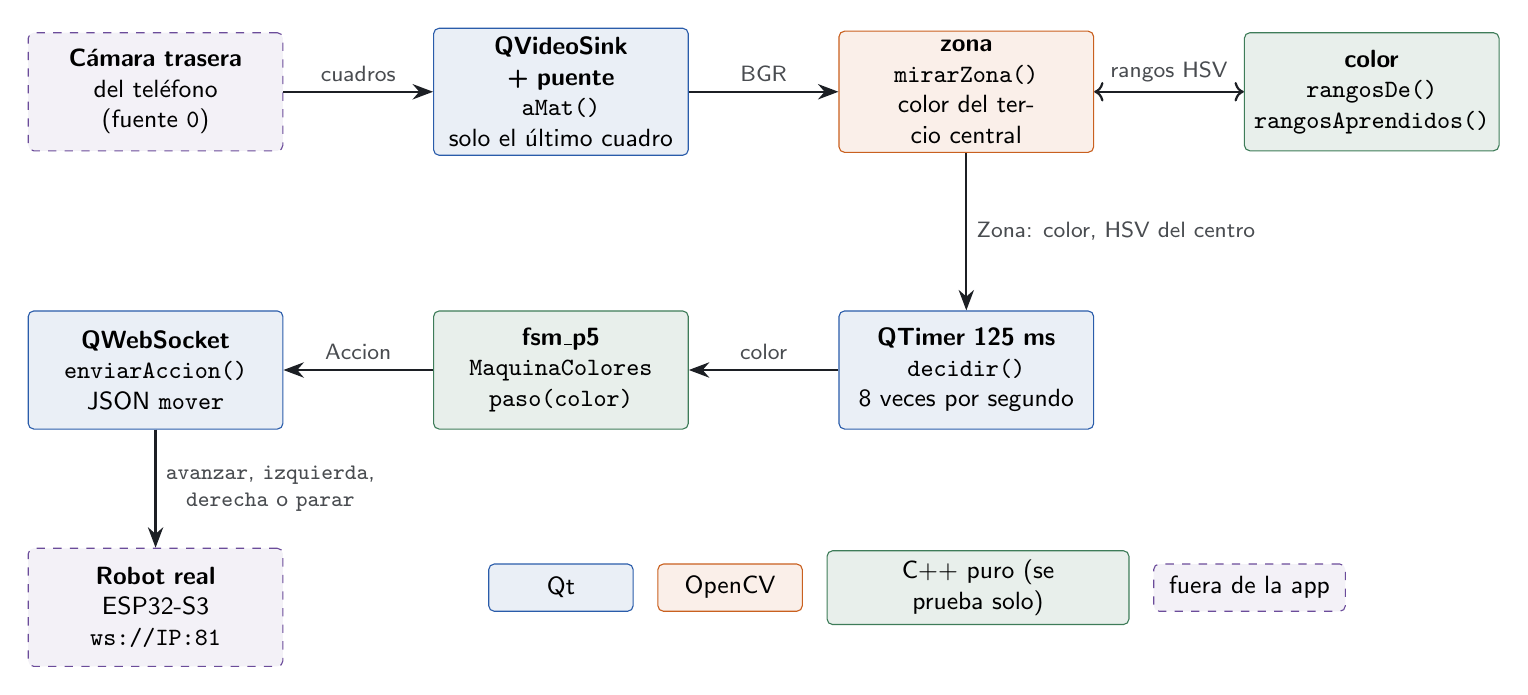
\begin{tikzpicture}[font=\sffamily\small,
  b/.style={draw=optoink, rounded corners=2pt, fill=white, minimum height=1.5cm, text width=3.0cm, align=center},
  qt/.style={b, draw=optosignal, fill=optosignal!10},
  cv/.style={b, draw=optoemit, fill=optoemit!10},
  pura/.style={b, draw=optoconfirm, fill=optoconfirm!12},
  ext/.style={b, draw=optodetect, fill=optodetect!8, dashed},
  fl/.style={-{Stealth[length=2.6mm]}, thick, optoink},
  et/.style={font=\sffamily\footnotesize, text=optoink!80, align=center}]
\node[ext] (cam) at (0,0) {\textbf{Cámara trasera}\\del teléfono\\(fuente \texttt{0})};
\node[qt, right=1.9cm of cam] (sink) {\textbf{QVideoSink + puente}\\\texttt{aMat()}\\solo el último cuadro};
\node[cv, right=1.9cm of sink] (zona) {\textbf{zona}\\\texttt{mirarZona()}\\color del tercio central};
\node[pura, right=1.9cm of zona] (color) {\textbf{color}\\\texttt{rangosDe()}\\\texttt{rangosAprendidos()}};
\draw[fl] (cam) -- node[et, above]{cuadros} (sink);
\draw[fl] (sink) -- node[et, above]{BGR} (zona);
\draw[fl, <->] (zona) -- node[et, above]{rangos HSV} (color);
\node[qt, below=2.0cm of zona] (timer) {\textbf{QTimer 125 ms}\\\texttt{decidir()}\\8 veces por segundo};
\node[pura, left=1.9cm of timer] (fsm) {\textbf{fsm\_p5}\\\texttt{MaquinaColores}\\\texttt{paso(color)}};
\node[qt, left=1.9cm of fsm] (ws) {\textbf{QWebSocket}\\\texttt{enviarAccion()}\\JSON \texttt{mover}};
\node[ext, below=1.5cm of ws] (robot) {\textbf{Robot real}\\ESP32-S3\\\texttt{ws://IP:81}};
\draw[fl] (zona) -- node[et, right]{Zona: color, HSV del centro} (timer);
\draw[fl] (timer) -- node[et, above]{color} (fsm);
\draw[fl] (fsm) -- node[et, above]{Accion} (ws);
\draw[fl] (ws) -- node[et, right]{\texttt{avanzar}, \texttt{izquierda},\\\texttt{derecha} o \texttt{parar}} (robot);
\node[qt, minimum height=0.6cm, text width=1.6cm, below=1.7cm of fsm] (l1) {Qt};
\node[cv, minimum height=0.6cm, text width=1.6cm, right=0.3cm of l1] (l2) {OpenCV};
\node[pura, minimum height=0.6cm, text width=3.6cm, right=0.3cm of l2] (l3) {C++ puro (se prueba solo)};
\node[ext, minimum height=0.6cm, text width=2.2cm, right=0.3cm of l3] (l4) {fuera de la app};
\end{tikzpicture}
\end{document}
